\documentclass[a4paper,openright,12pt]{book}
\usepackage[spanish]{babel} % espanol
\usepackage{fancyhdr}
\usepackage{lastpage}
\usepackage{graphicx} % graficos
\usepackage{hyperref}
\usepackage[utf8]{inputenc}
\usepackage{enumerate}


% nivel que se numera y aparece en el indice
\setcounter{secnumdepth}{3}
\setcounter{tocdepth}{3}

% quitar el 0.
\renewcommand\thesection{\arabic{section}}

% tabla de contenidos como seccion
\makeatletter
\renewcommand\tableofcontents{
    \section*{{Tabla de contenidos} %linea importante
        \@mkboth{
           \MakeUppercase\contentsname}{\MakeUppercase\contentsname}}
    \@starttoc{toc}
    }
\makeatother

% bibliografia como seccion
\makeatletter
\renewenvironment{thebibliography}[1]{
     \section*{Bibliografía} %linea importante
      \@mkboth{\MakeUppercase\bibname}{\MakeUppercase\bibname}
      \list{\@biblabel{\@arabic\c@enumiv}}
           {\settowidth\labelwidth{\@biblabel{#1}}
            \leftmargin\labelwidth
            \advance\leftmargin\labelsep
            \@openbib@code
            \usecounter{enumiv}
            \let\p@enumiv\@empty
            \renewcommand\theenumiv{\@arabic\c@enumiv}}
      \sloppy
      \clubpenalty4000
      \@clubpenalty \clubpenalty
      \widowpenalty4000
      \sfcode`\.\@m}
     {\def\@noitemerr
       {\@latex@warning{Empty `thebibliography' environment}}
      \endlist}
\makeatother

% aqui definimos el encabezado
\lhead[\thepage/\pageref{LastPage}]{}
\chead[Informe]{Informe}
\rhead[]{\thepage/\pageref{LastPage}}
\renewcommand{\headrulewidth}{0.5pt}

% aqui definimos el pie de pagina
\lfoot[EPIS]{Base de Datos II}
\cfoot[\today]{\today}
\rfoot[Base de Datos II]{EPIS}
\renewcommand{\footrulewidth}{0.5pt}

\pagestyle{fancy} 

% margenes
\setlength{\oddsidemargin}{5mm}
\setlength{\evensidemargin}{5mm}

\begin{document}

\begin{titlepage}
\begin{center}
\begin{figure}[htb]
\begin{center}

\includegraphics[width=4cm]{./images/upt}
\end{center}
\end{figure}

UNIVERSIDAD PRIVADA DE TACNA\\
\vspace*{0.10in}
FACULTAD DE INGENIERIA\\
Escuela Profesional de Ingeniería de Sistemas\\
\vspace*{0.2in}
\begin{large}
TEMA : \\
\end{large}
\vspace*{0.2in}
\begin{Large}
\textbf{Trabajo Final de Unidad II - Guía de Instalación y Configuración de Base de Datos} \\
\end{Large}
\vspace*{0.3in}
\begin{large}
DOCENTE: PATRICK CUADROS QUIROGA\\
\end{large}
\vspace*{0.3in}
\rule{80mm}{0.1mm}\\
\vspace*{0.1in}
\begin{large}
PRESENTADO POR: \\
Jose Luis Condori Choquecota \\
Elisban Vilca Mamani\\


\end{large}
\rule{80mm}{0.1mm}\\
\begin{large}
2017\\
\end{large}
\end{center}
\end{titlepage}


\tableofcontents
\pagenumbering{arabic}
\lhead[\thepage/\pageref{LastPage}]{\thesection. Tabla de contenidos}
\rhead[\thesection. Tabla de contenidos]{\thepage/\pageref{LastPage}}
\newpage



\section{Oracle Linux modo Terminal}\label{se:nudo}
\lhead[\thepage/\pageref{LastPage}]{\thesection. Nudo}
\rhead[\thesection. Nudo]{\thepage/\pageref{LastPage}}

Paso 1: Una vez iniciado sesion con el usuario root abrimos una terminal ejecutamos el comando, lo que va hacer este comando es instalar repositorios que son necesarios para la instalacion de oracle database
\begin{center}
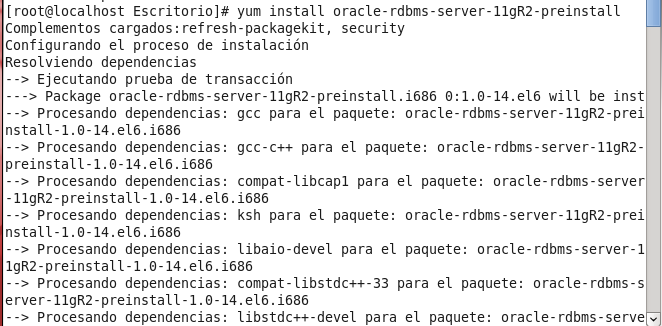
\includegraphics[width=15cm]{./oracle linux/1.png}
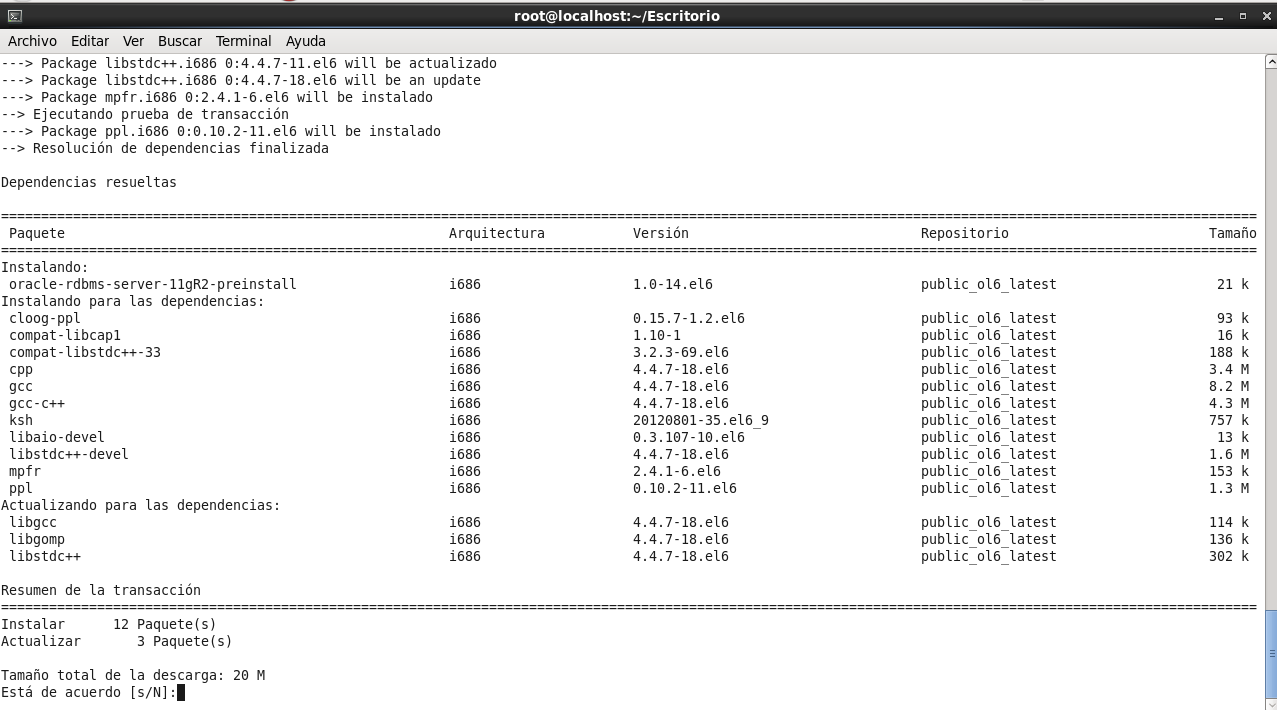
\includegraphics[width=15cm]{./oracle linux/2.png}
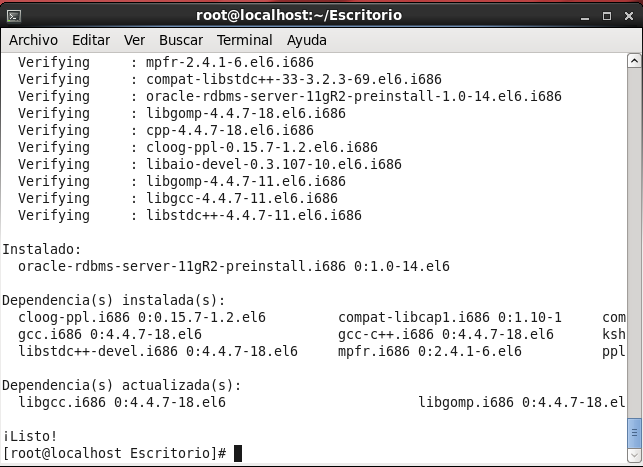
\includegraphics[width=15cm]{./oracle linux/3.png}
\end{center}

Paso 2 : Una vez instalada todos los repositorios faltantes Creamos la carpeta donde se instalara los db de oracle

\begin{center}
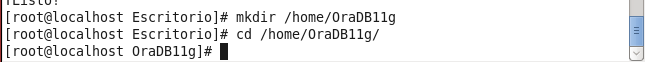
\includegraphics[width=15cm]{./oracle linux/4.png}
\end{center}
Paso 3 : Montamos un usb con el instalador en este caso tenemos el instaldor en dos partes en archivos zip,una vez montado el usb copiamos los archivos a la carpeta creada anteriormente “/home/OraDB11g”.

\begin{center}
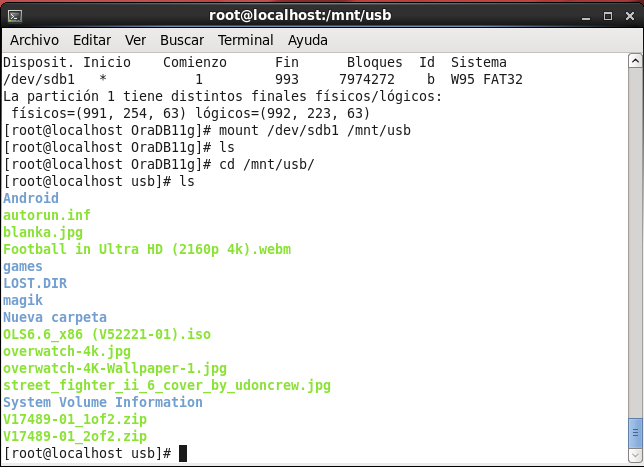
\includegraphics[width=15cm]{./oracle linux/5.png}
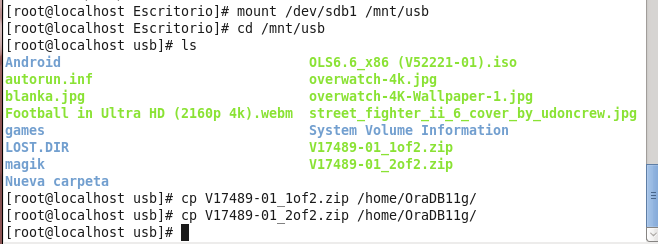
\includegraphics[width=15cm]{./oracle linux/6.png}
\end{center}

Paso 4 : Una vez copiado los archivos nos dirigimos a la carpeta “/home/OraDB11g”  para extraer el instalador
\begin{center}
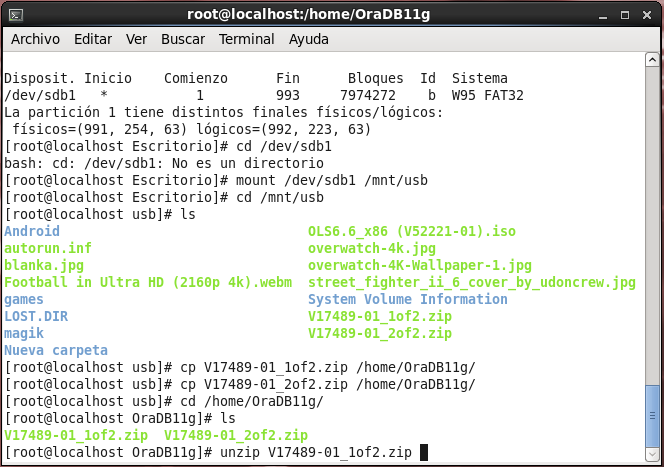
\includegraphics[width=15cm]{./oracle linux/7.png}
\end{center}
Paso 5 : Una vez extraida se creara un carpeta “database”.

\begin{center}
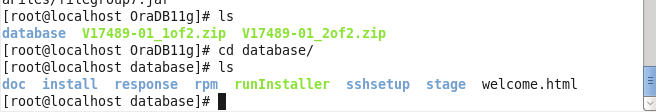
\includegraphics[width=15cm]{./oracle linux/8.png}
\end{center}
Paso 6 : Ahora para ejecutar el “runInstaller” debemos iniciar sesion con el usuario ”oracle” para eso de asiganamos una contraseña con el comando “passwd”.
\begin{center}
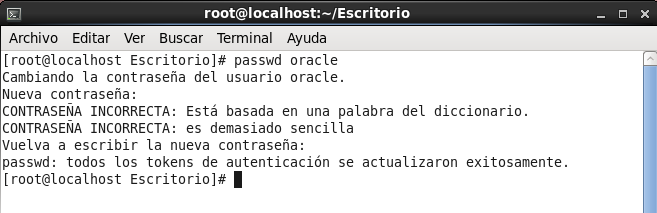
\includegraphics[width=15cm]{./oracle linux/9.png}
\end{center}

Paso 7 : Luego iniciamos sesion y nos dirimos a la carpeta donde se encuentra el instalador y ejecutamos “runInstaller”.

\begin{center}
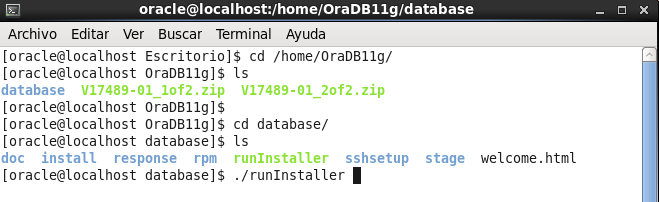
\includegraphics[width=15cm]{./oracle linux/10.png}
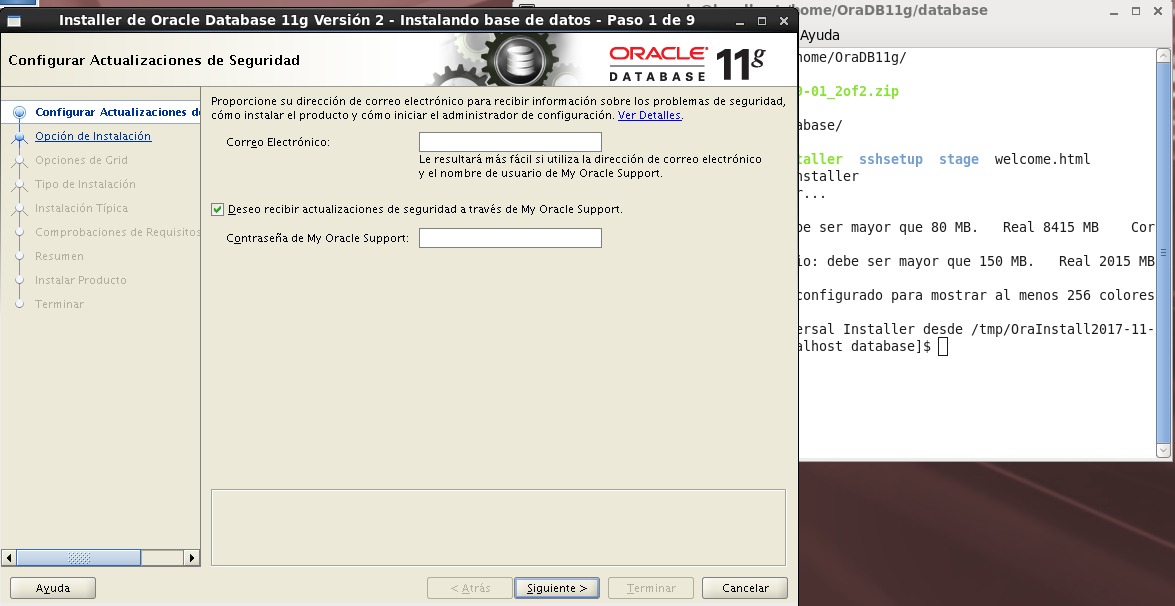
\includegraphics[width=15cm]{./oracle linux/11.png}
Proporcionamos una direccion de correo electrnico para recibir informacion sobre los problemas de seguridad.\\
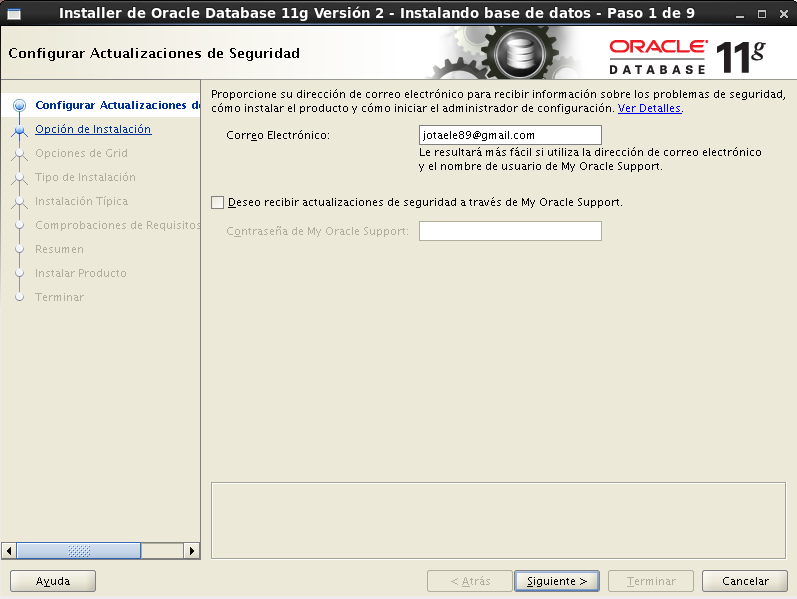
\includegraphics[width=15cm]{./oracle linux/12.png}
Seleccionamos cualquiera de las opciones.\\
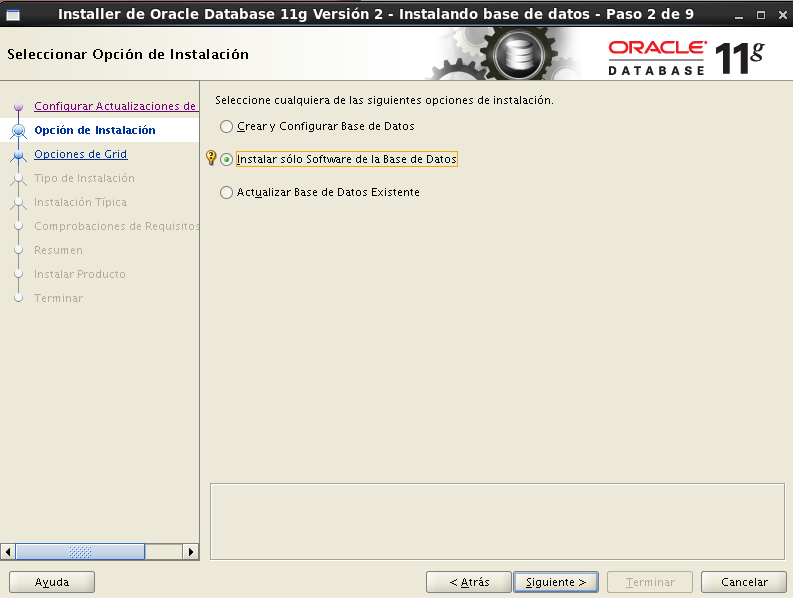
\includegraphics[width=15cm]{./oracle linux/13.png}
Seleccionamos el tipo de instalacion de base de datos.\\
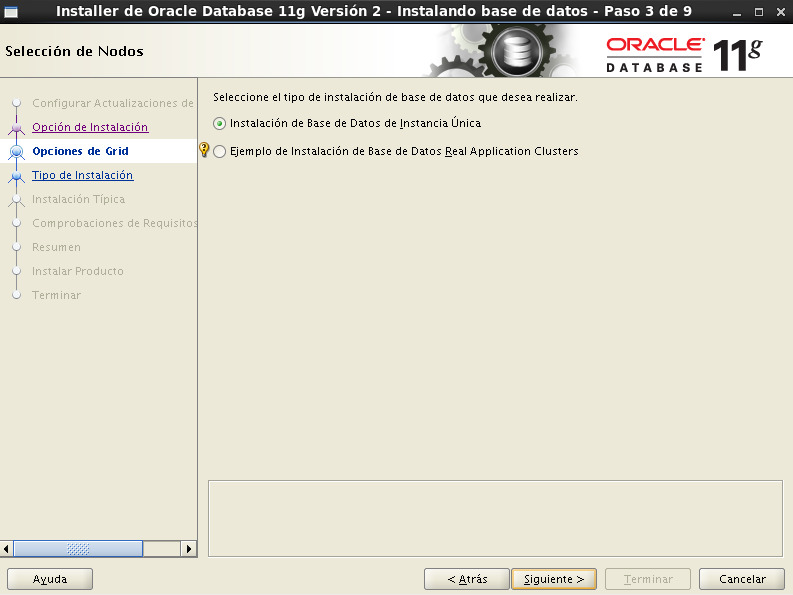
\includegraphics[width=15cm]{./oracle linux/14.png}
Seleccionamos los idiomas en que se ejecutara el producto.\\
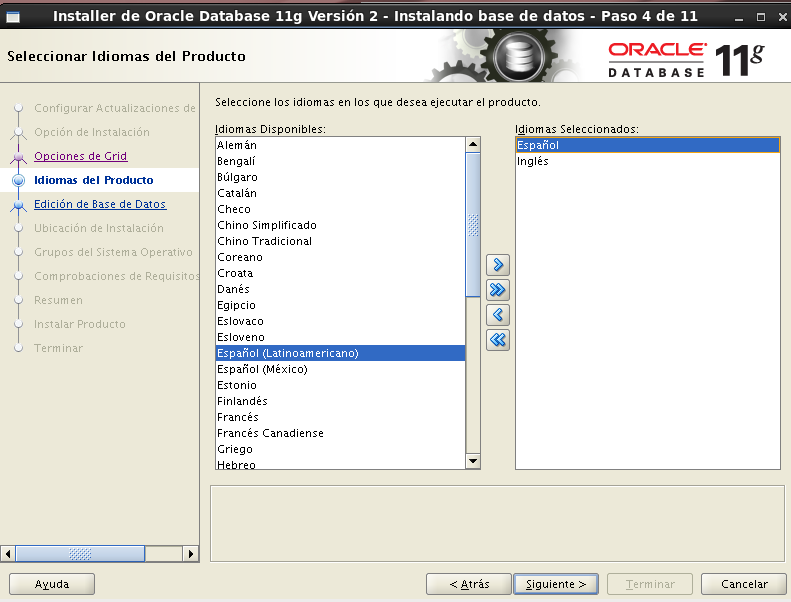
\includegraphics[width=15cm]{./oracle linux/15.png}
Seleccionamos la edicion de base de datos que deseamos instalar.\\
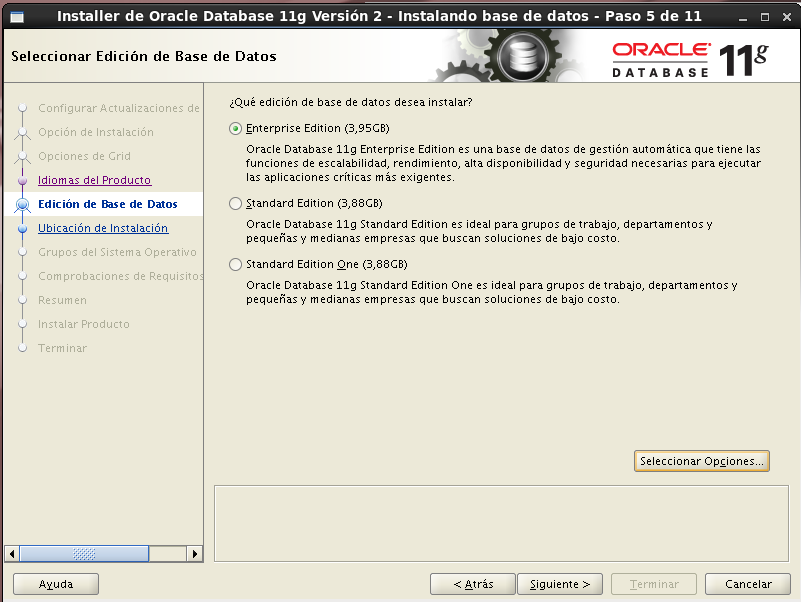
\includegraphics[width=15cm]{./oracle linux/16.png}
Especificamos la ruta de acceso al direcctorio a la base de Oracle.\\
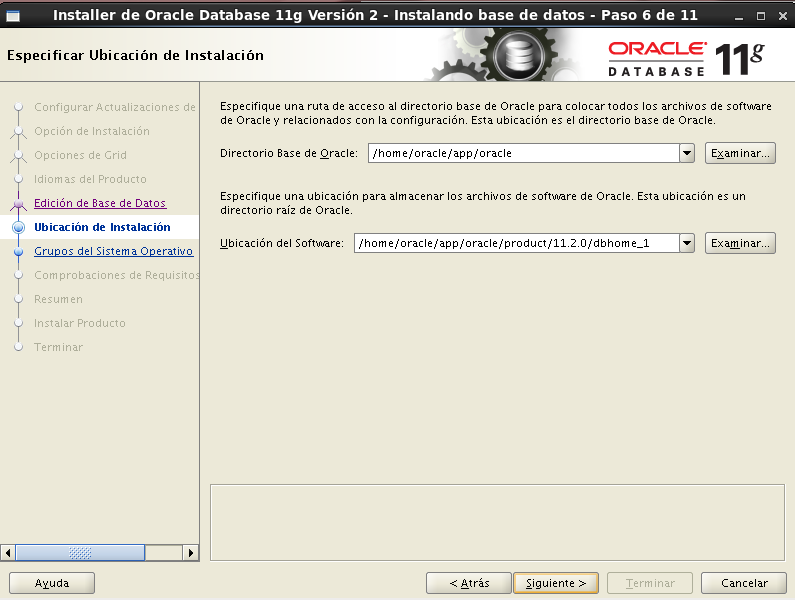
\includegraphics[width=15cm]{./oracle linux/17.png}
Especificamos un directorio para los archivos de instalacion.\\
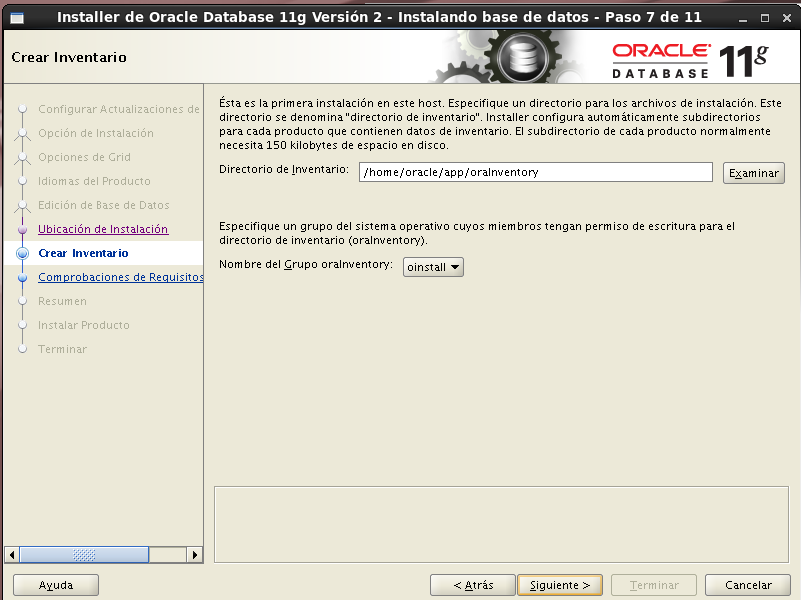
\includegraphics[width=15cm]{./oracle linux/18.png}
Otorgamos los permisos necesarios.\\
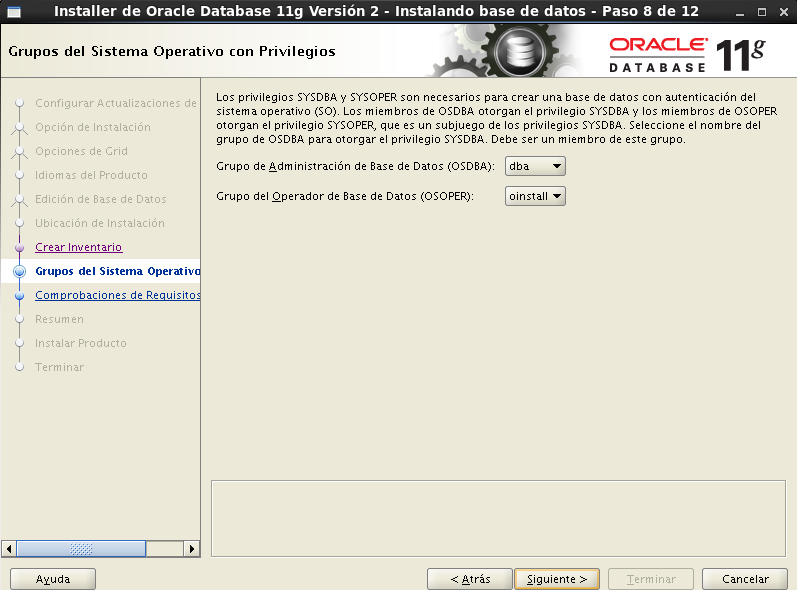
\includegraphics[width=15cm]{./oracle linux/19.png}
Verificara los requisitos minimos de instalacion y configuracion.\\
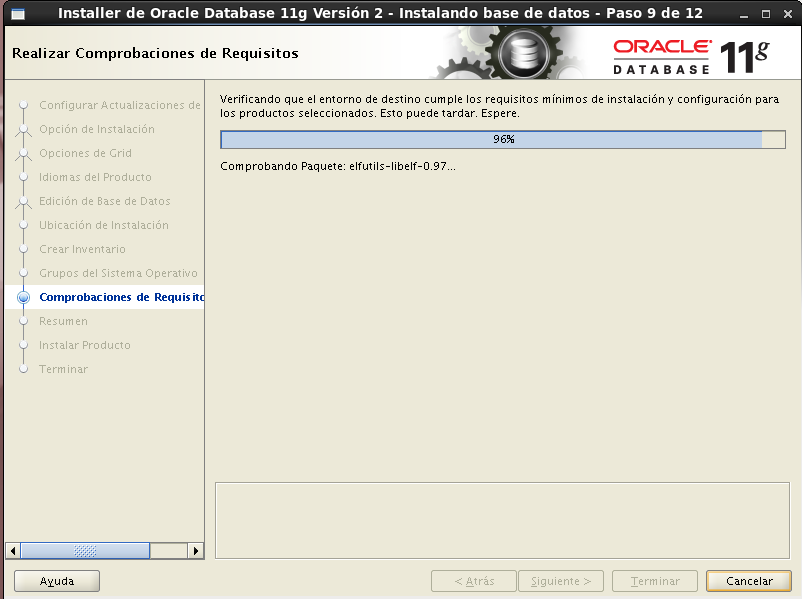
\includegraphics[width=15cm]{./oracle linux/20.png}
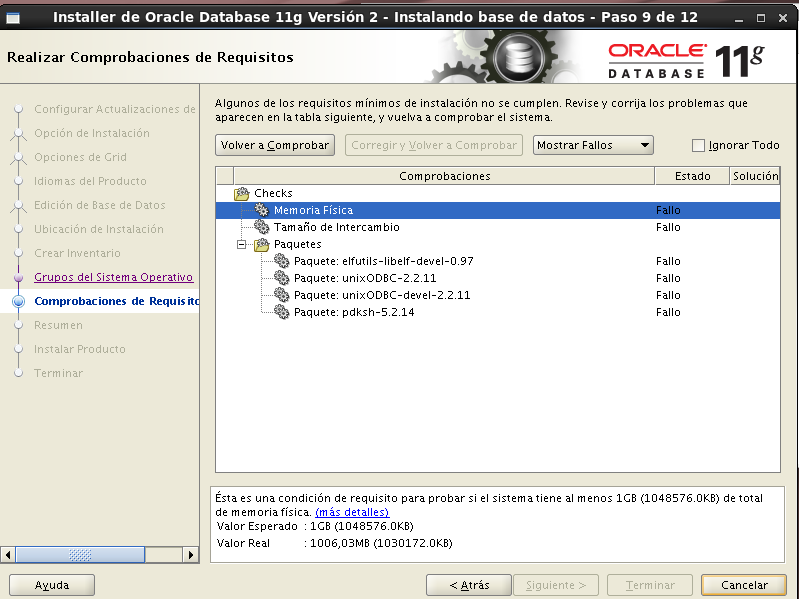
\includegraphics[width=15cm]{./oracle linux/21.png}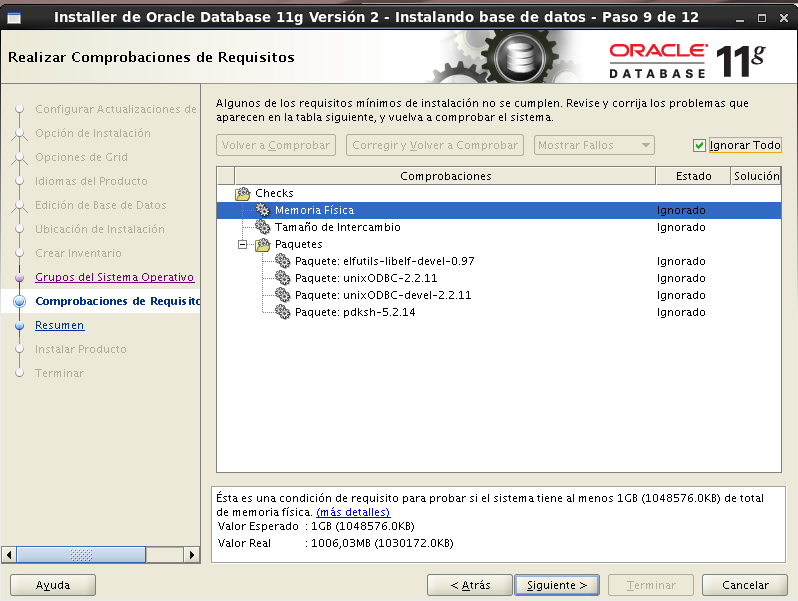
\includegraphics[width=15cm]{./oracle linux/22.png}
Nos mostrara el resumen de lo que vamos a instalar.\\
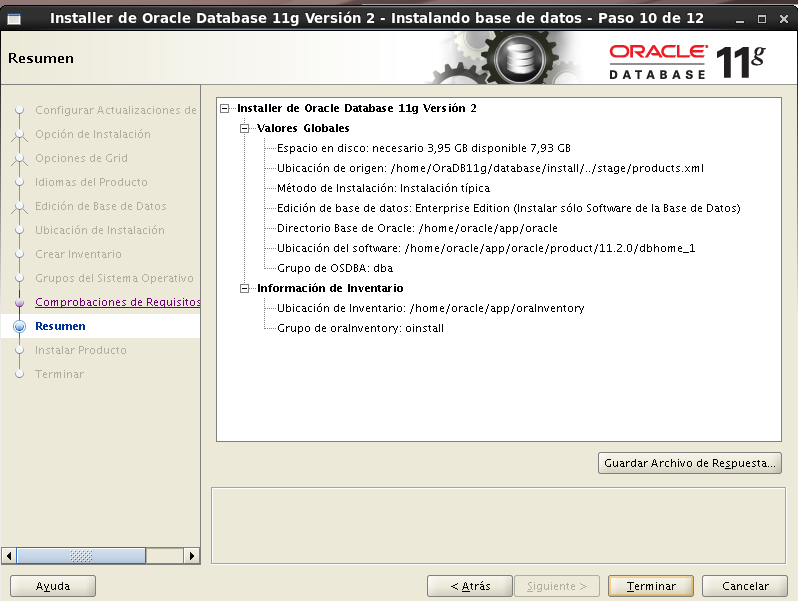
\includegraphics[width=15cm]{./oracle linux/23.png}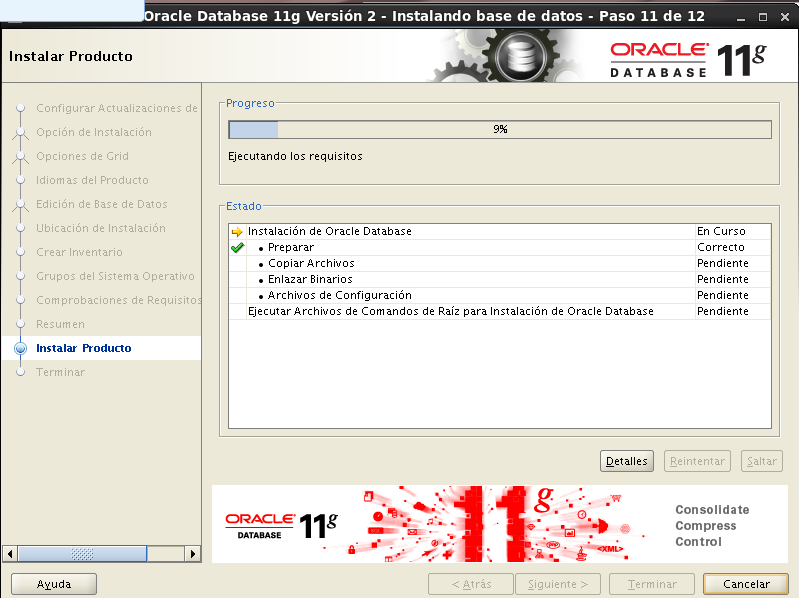
\includegraphics[width=15cm]{./oracle linux/24.png}
Antes de terminar la instalacion nos saltara un ventana donde nos indica que antes de terminar la instalacion debemos ejecutar algunos scripts
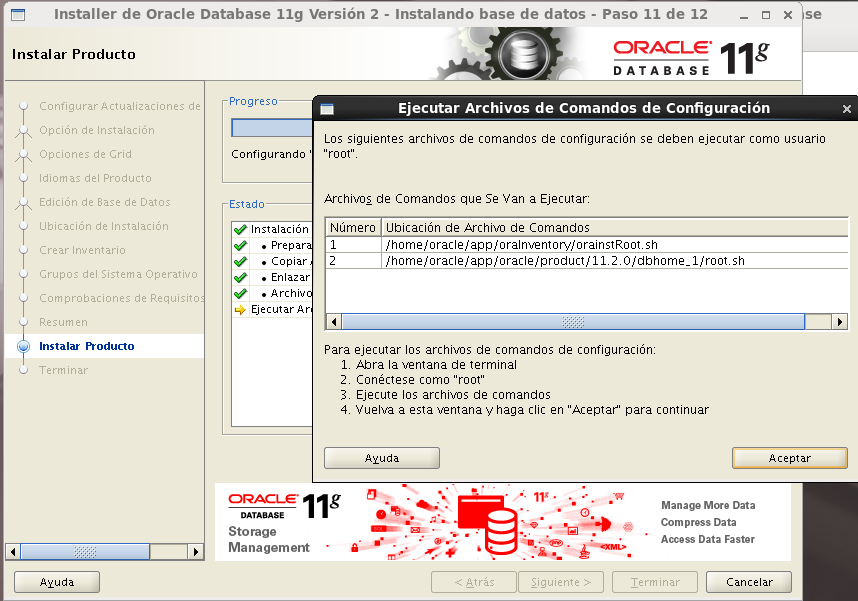
\includegraphics[width=15cm]{./oracle linux/25.png}
Abrimos otra terminal e iniciamos sesion con el usuario "root" y ejecutamos el primer script
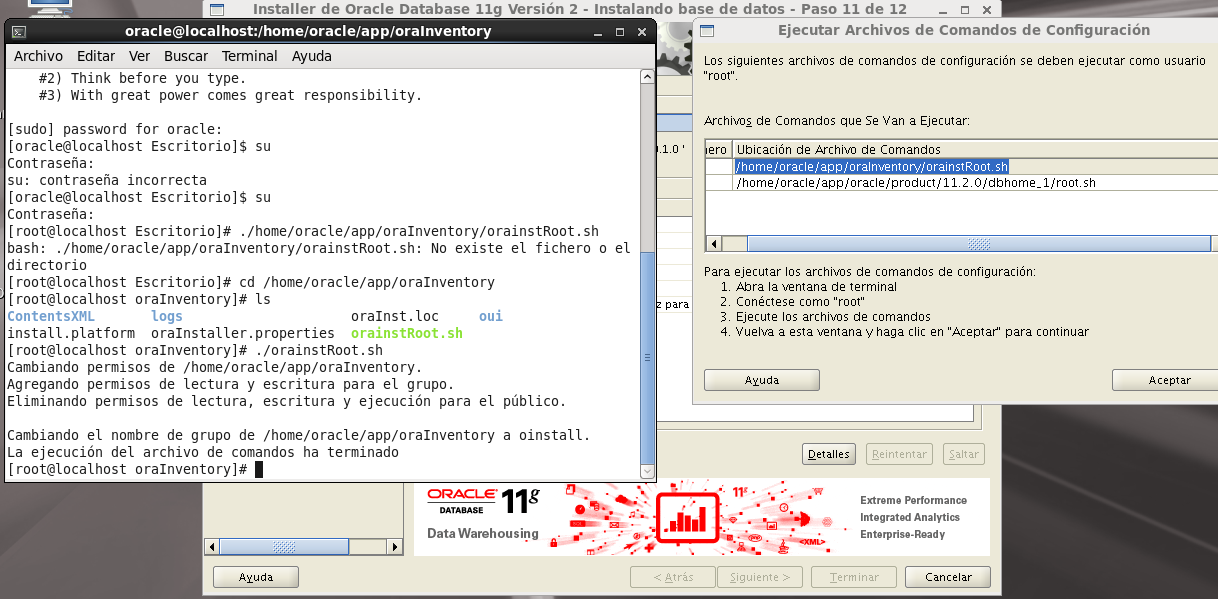
\includegraphics[width=15cm]{./oracle linux/27.png}
Ahora vamos con el segundo  con esto bastara y terminara la instalacion
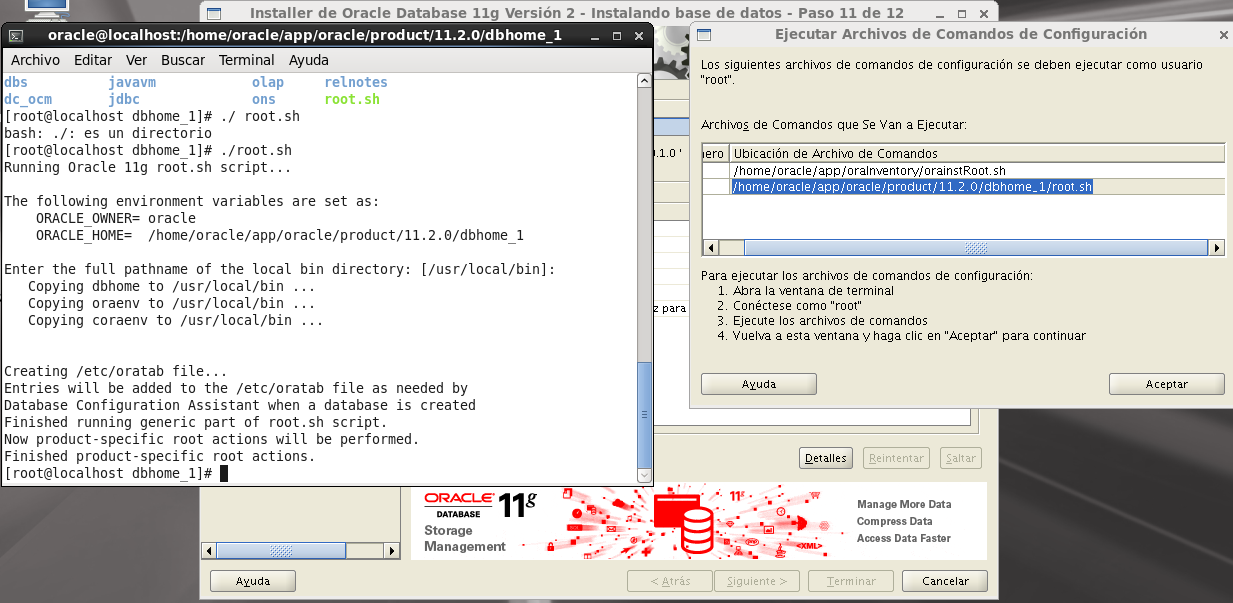
\includegraphics[width=15cm]{./oracle linux/28.png}

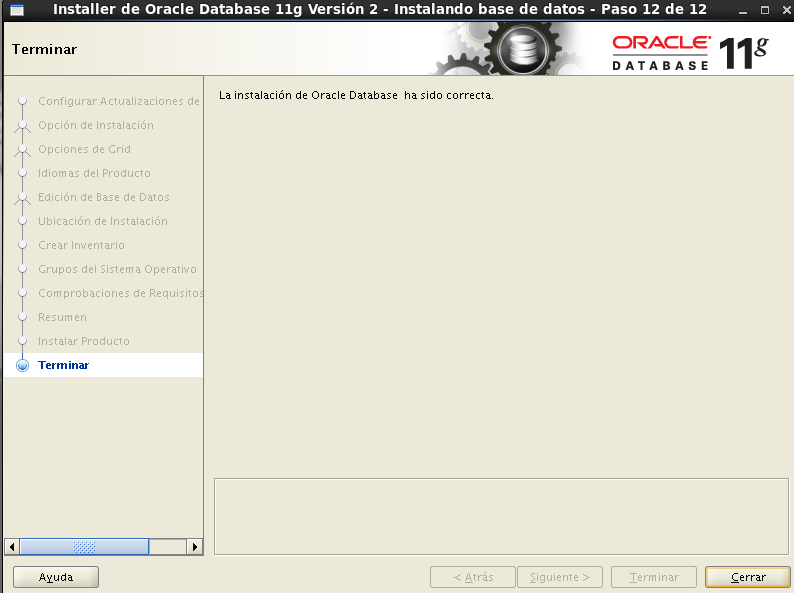
\includegraphics[width=15cm]{./oracle linux/29.png}
\end{center}

\section{Windows Server }
\lhead[\thepage/\pageref{LastPage}]{\thesection. Nudo}
\rhead[\thesection. Nudo]{\thepage/\pageref{LastPage}}

Pasos de la Instalación\\

Paso 1: El instalador de la base de datos Oracle 11g versión 2 archivos se divide en dos archivos zip.   Es necesario descargar ambos archivos y luego extraerlas ambas en una carpeta por ejemplo instaladorOracle o con cualquier otro nombre.\\
\begin{center}
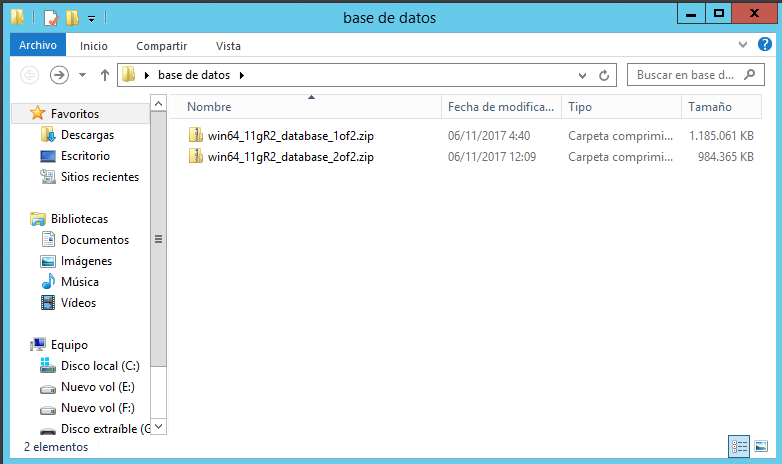
\includegraphics[width=15cm]{./windows server/1.png}
\end{center}

Paso 2: Luego de descomprimir ambos archivos el directorio quedará de la siguiente forma.\\
\begin{center}
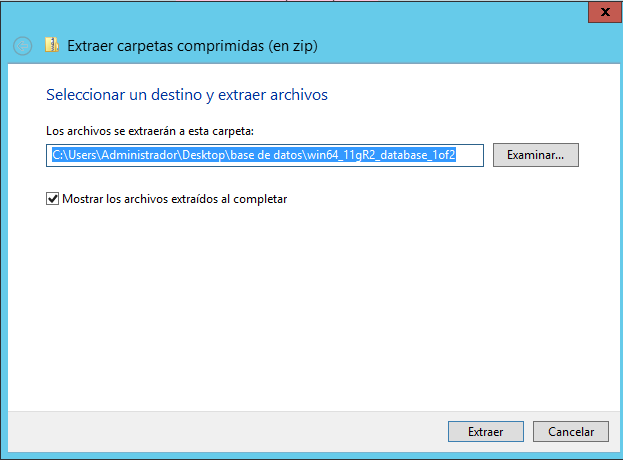
\includegraphics[width=15cm]{./windows server/2.png}
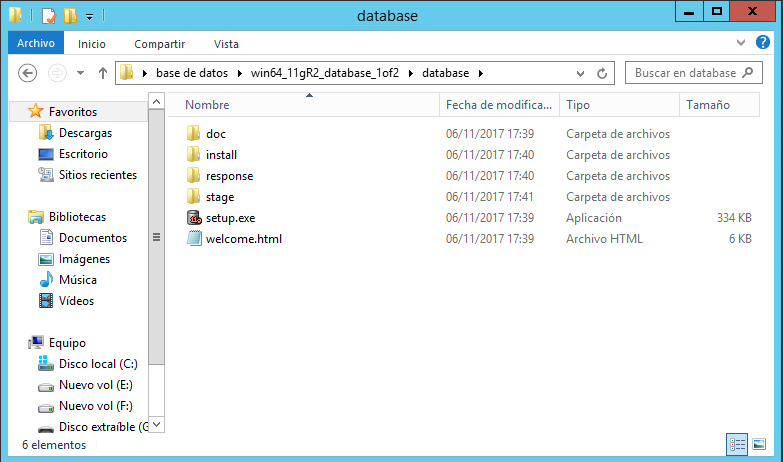
\includegraphics[width=15cm]{./windows server/3.png}
\end{center}


Paso 3: Dentro de la carpeta ejecutar el archivo setup.exe y se abrirá la ventana del  Oracle Universal Installer, que puede permanecer unos segundos.\\ 
\begin{center}
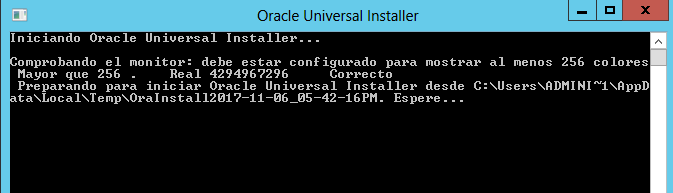
\includegraphics[width=15cm]{./windows server/4.png}
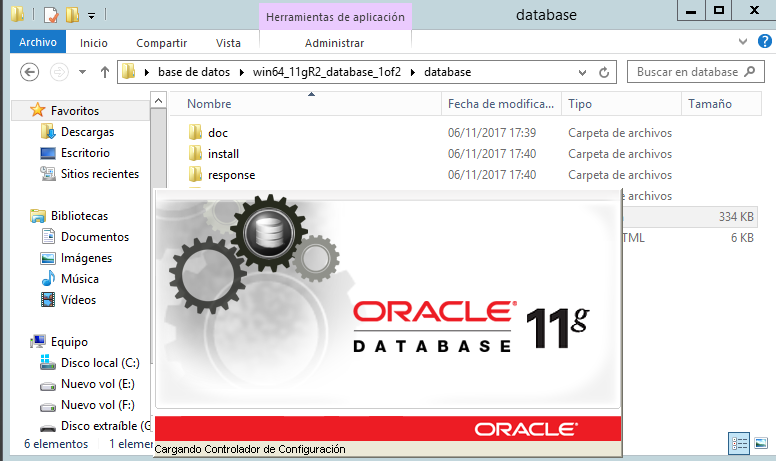
\includegraphics[width=15cm]{./windows server/5.png}
\end{center}

Paso 4: En la siguiente pantalla pide proporcionar una dirección de correo electrónico para recibir información sobre los problemas de seguridad.  En este caso desactivamos la casilla de recibir actualizaciones de seguridad a través del soporte de Oracle.  
\begin{center}
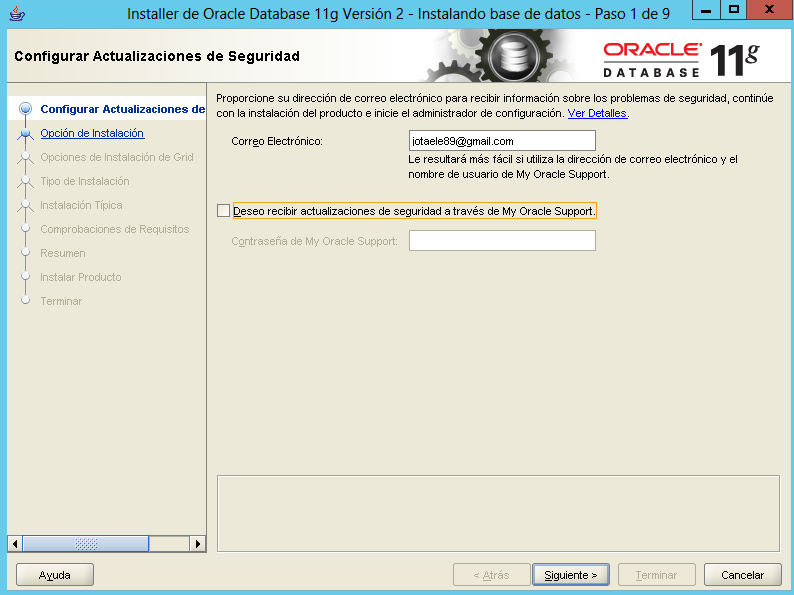
\includegraphics[width=15cm]{./windows server/6.png}
\end{center}
Paso 5 En nuestro caso, puesto que se trata de una instalación desde cero marcaremos "Crear y Configurar Base de Datos":
\begin{center}
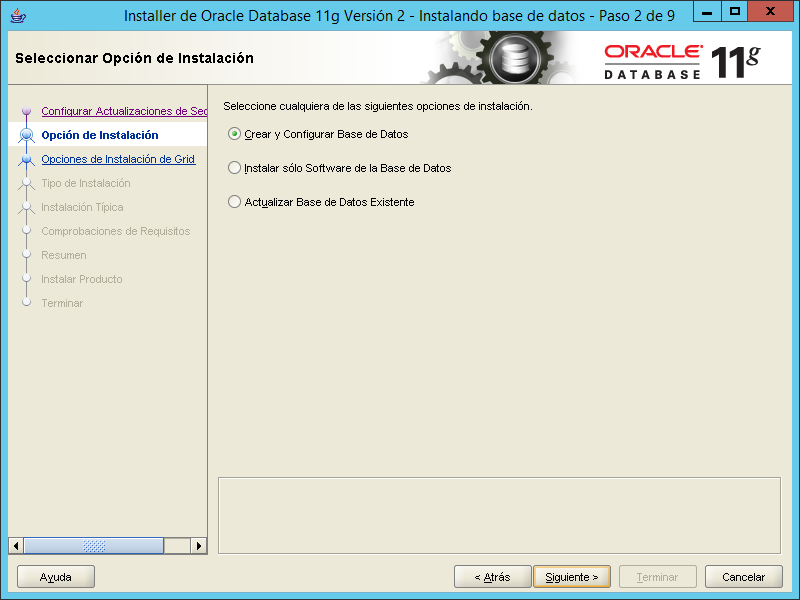
\includegraphics[width=15cm]{./windows server/7.png}
\end{center}


Paso 6: Seleccionar "Clase de Escritorio", que es una instalación bastante más sencilla pues el asistente pedirá una configuración mínima y el resto de parámetros avanzados los establecerá de forma automática. Este método es más sencillo de instalar aunque se tendrá menor control sobre la instalación
\begin{center}
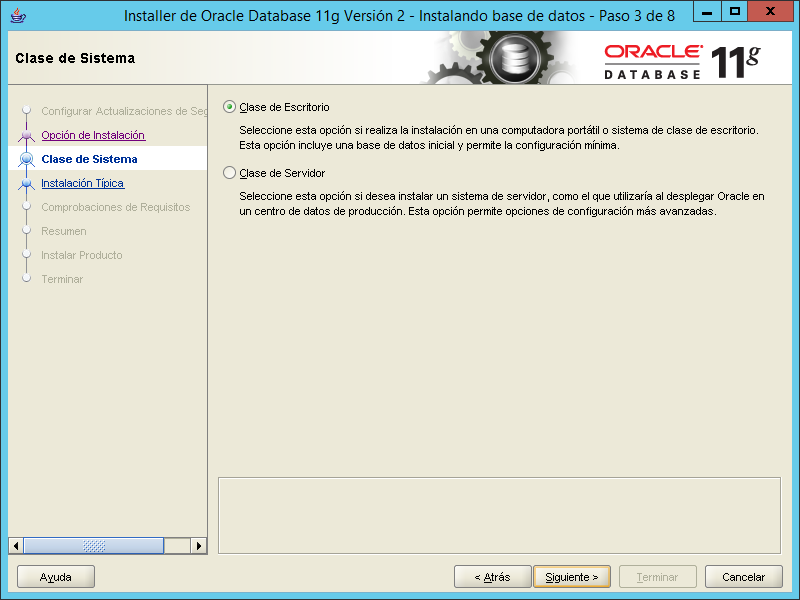
\includegraphics[width=15cm]{./windows server/8.png}
\end{center}


Paso 7: A continuación indicaremos los siguientes datos:

Directorio Base de Oracle: Ubicación del directorio raíz de Oracle
Ubicación del Software: Destino de los archivos de la instalación de Oracle.
Ubicación de Archivos de Base de Datos: Ubicación de los archivos de datos que almacenará la base de datos.
Edición de Base de Datos: Tipo de instalación, a elegir entre "Enterprise Edition", "Standar Edition", "Standard Edition One", "Personal Edition". 
Juego de Caracteres: Juego de caracteres que se asignará a la base de datos.
Nombre de la Base de Datos Global: SID que tendrá la base de datos para identificarla unívocamente de otras, por defecto "orcl".
Contraseña del Administrador: contraseña para el usuario "system" y "sys".
Confirmar Contraseña y clic en siguiente.
\begin{center}
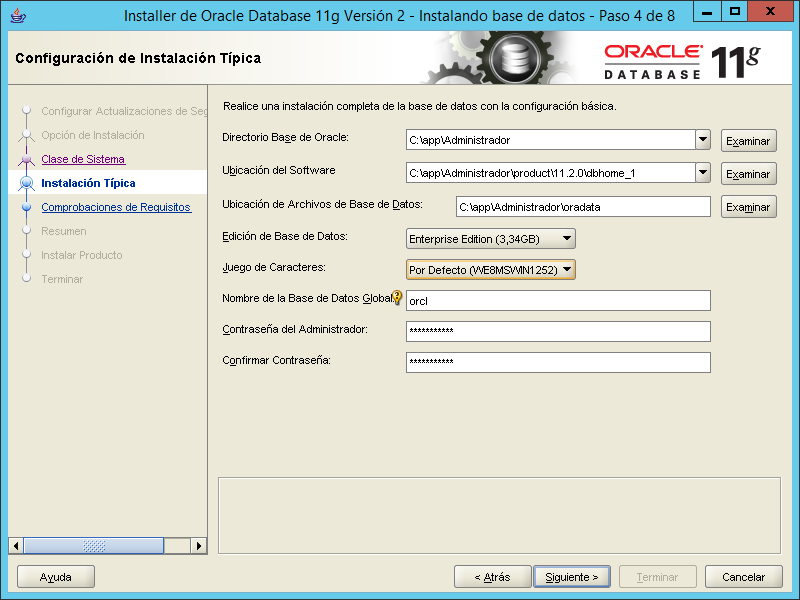
\includegraphics[width=15cm]{./windows server/9.png}
\end{center}


Paso 8: Se iniciará la verificación de los requisitos mínimos por parte del asistente, comprobará si la configuración y el hardware de nuestro equipo cumple con los requisitos mínimos y mostrará la ventana resumen de las opciones seleccionadas para la instalación. Clic en terminar para continuar.
\begin{center}
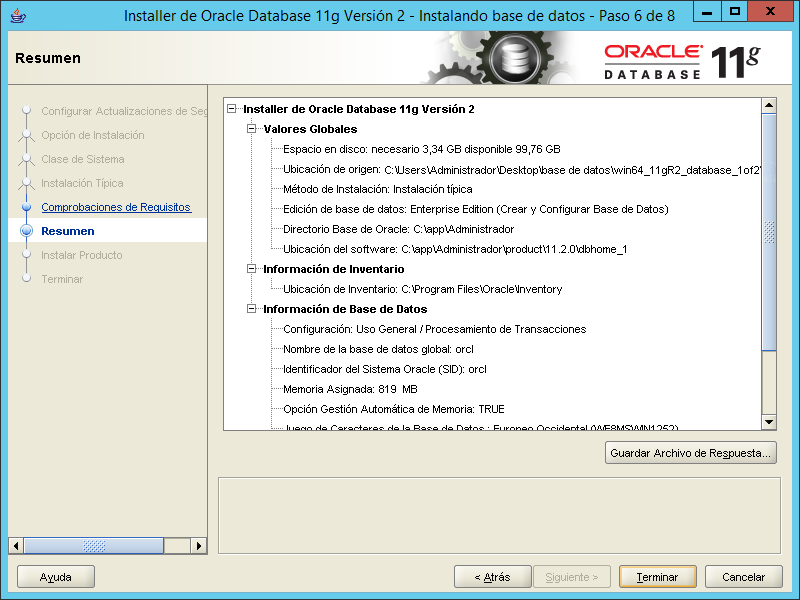
\includegraphics[width=15cm]{./windows server/10.png}
\end{center}

Paso 9: Es la pantalla principal de instalación, demorá entre 10 a 15 minutos. El asistente nos mostrará el progreso de la instalación así como las tareas realizadas (instalación de Oracle Database, preparar sistema, copiar archivos, crear archivos de configuración, configurar Oracle Database, crear base de datos)
\begin{center}
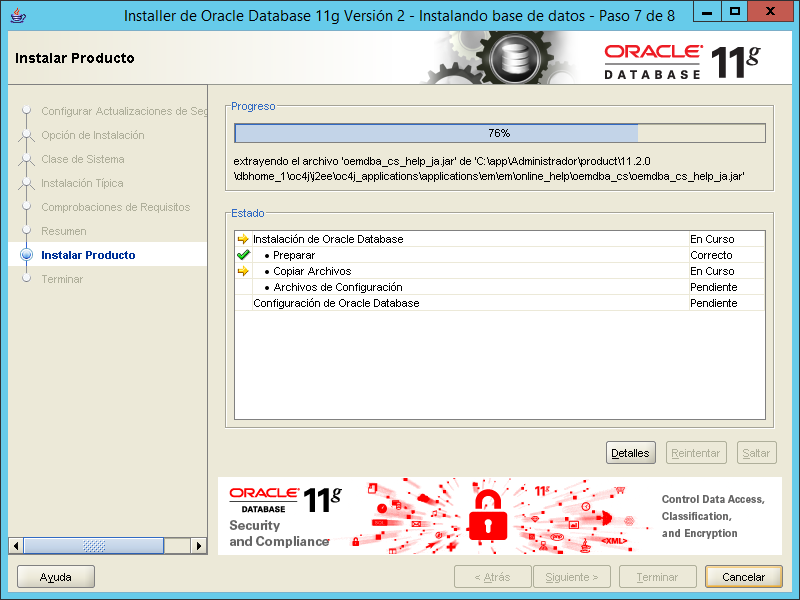
\includegraphics[width=15cm]{./windows server/11.png}
\end{center}


Paso 10: Al final de la instalación de Oracle 11g se iniciará el proceso de creación de la base de datos (copia de archivos, crear e iniciar instancia de oracle):
\begin{center}
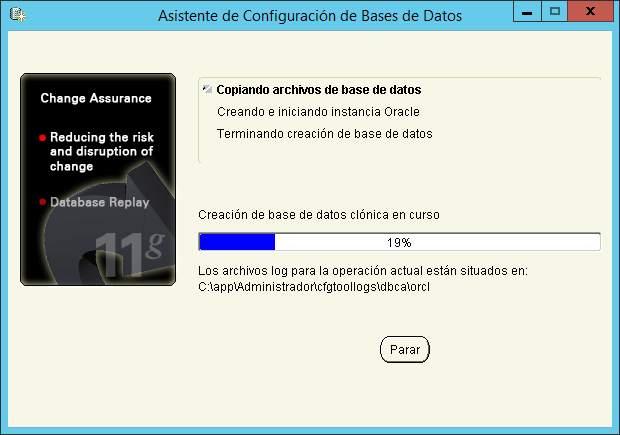
\includegraphics[width=15cm]{./windows server/12.png}
\end{center}


Paso 11: El asistente de Configuración de Bases de Datos nos mostrará la ventana desde la que podremos acceder a la gestión de contraseñas de los usuarios y en la que nos mostrará la URL de administración para acceso a Oracle Database Control, por defecto:
https://localhost:1158/em
\begin{center}
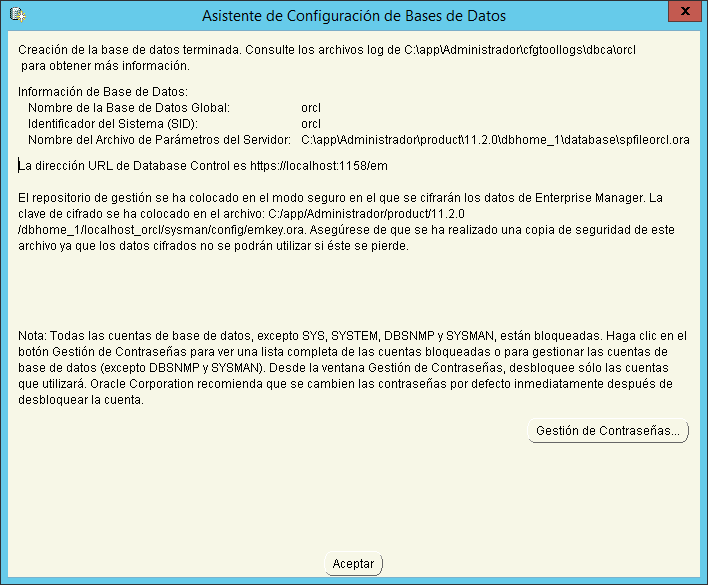
\includegraphics[width=15cm]{./windows server/13.png}
\end{center}


Paso 12: Por último la ventana indicando que la instalación de oracle ha sido correcta.
\begin{center}
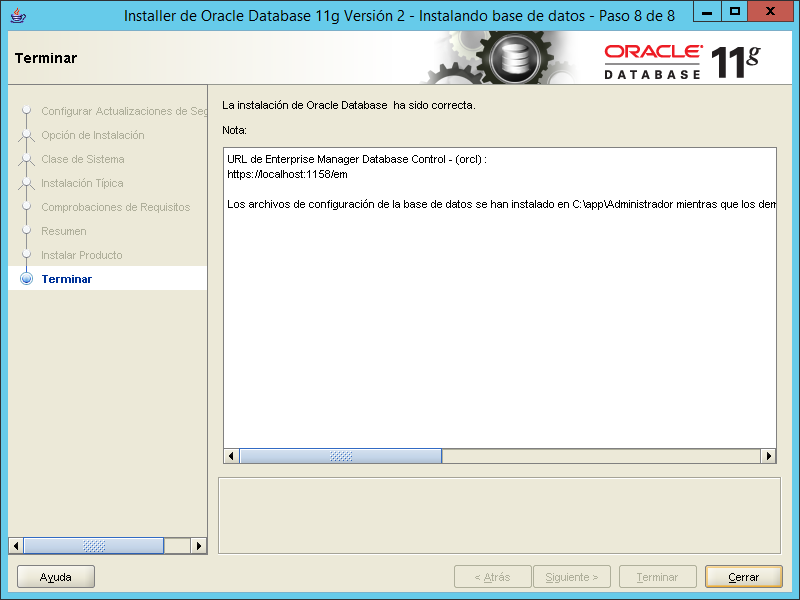
\includegraphics[width=15cm]{./windows server/14.png}
\end{center}

\end{document}
